\documentclass[12pt,a4paper]{article}

\usepackage[spanish,es-tabla]{babel}
\usepackage{geometry}
\usepackage{graphicx}
\usepackage{booktabs}
\usepackage{tabularx}
\usepackage{longtable}
\usepackage{array}
\usepackage{enumitem}
\usepackage{hyperref}
\usepackage{xcolor}
\usepackage{float}
\usepackage{fancyhdr}
\usepackage{parskip}
\usepackage{setspace}

\geometry{margin=2.5cm}
\setstretch{1.15}
\emergencystretch=2em
\graphicspath{{figures/}}
\setlist[itemize]{leftmargin=1.5em}
\setlength{\headheight}{15pt}

\hypersetup{
  colorlinks=true,
  linkcolor=blue!50!black,
  urlcolor=blue!50!black,
  pdftitle={Documentacion tecnica - Trivia Crack Quiz Multiplayer},
  pdfauthor={Proyecto Juego Multijugador Paradigma Funcional}
}

\pagestyle{fancy}
\fancyhf{}
\fancyhead[L]{Trivia Crack Quiz Multiplayer}
\fancyhead[R]{Documentacion tecnica}
\fancyfoot[C]{\thepage}

\begin{document}

\begin{titlepage}
  \centering
  \vspace*{2cm}

  {\Huge \textbf{Documentacion Tecnica del Proyecto}\par}
  \vspace{0.5cm}
  {\LARGE Trivia Crack Quiz Multiplayer\par}
  \vspace{1.5cm}

  {\large Juego multijugador desarrollado con Elixir, Phoenix LiveView y OTP\par}
  \vspace{1cm}

  {\large \textbf{Repositorio}\par}
  {\small \url{https://github.com/aaabriceno/Juego_Multijugador_Paradigm_Funcional_QUIZZ.git}\par}
  \vspace{0.5cm}
  {\large \textbf{Framework principal:} Phoenix 1.8 con LiveView\par}
  \vspace{0.2cm}
  {\large \textbf{Paradigma concurrente:} Modelo de actores sobre Erlang/OTP\par}
  \vspace{0.2cm}
  {\large \textbf{Documento complementario:} \path{docs/guia_instalacion_local.md}\par}

  \vfill

  {\large Junio 2026\par}
\end{titlepage}

\tableofcontents
\newpage

\section{Vision general del proyecto}

Trivia Crack Quiz Multiplayer es una aplicacion web multijugador en tiempo real
que permite crear salas independientes de trivia, unir jugadores desde varios
navegadores y mantener el puntaje sincronizado sin recargas de pagina. El
proyecto se construyo con Elixir y Phoenix LiveView, y adopta el modelo de
actores de Erlang/OTP para que cada sala de juego exista como un proceso
aislado con estado propio.

El sistema cubre tres objetivos tecnicos centrales:

\begin{itemize}
  \item administrar varias salas en paralelo sin compartir memoria entre ellas;
  \item mantener una experiencia en tiempo real mediante PubSub y LiveView;
  \item separar la logica funcional pura del juego de los efectos asociados a
  procesos, temporizadores, supervision y comunicacion con clientes.
\end{itemize}

Desde la perspectiva del usuario, el flujo principal se compone de cuatro
pantallas: lobby general, creacion de sala, partida activa y tablero
espectador. Desde la perspectiva tecnica, esas vistas son clientes LiveView que
delegan toda la coordinacion del juego a procesos OTP y a un motor funcional de
reglas.

\section{Arquitectura general y estructura del juego}

La aplicacion sigue la organizacion habitual de un proyecto Phoenix: el dominio
del juego vive en \texttt{lib/trivia\_crack\_quiz/} y la capa web en
\texttt{lib/trivia\_crack\_quiz\_web/}. La Figura~\ref{fig:estructura-juego}
resume como se relacionan sus piezas principales.

\begin{figure}[H]
  \centering
  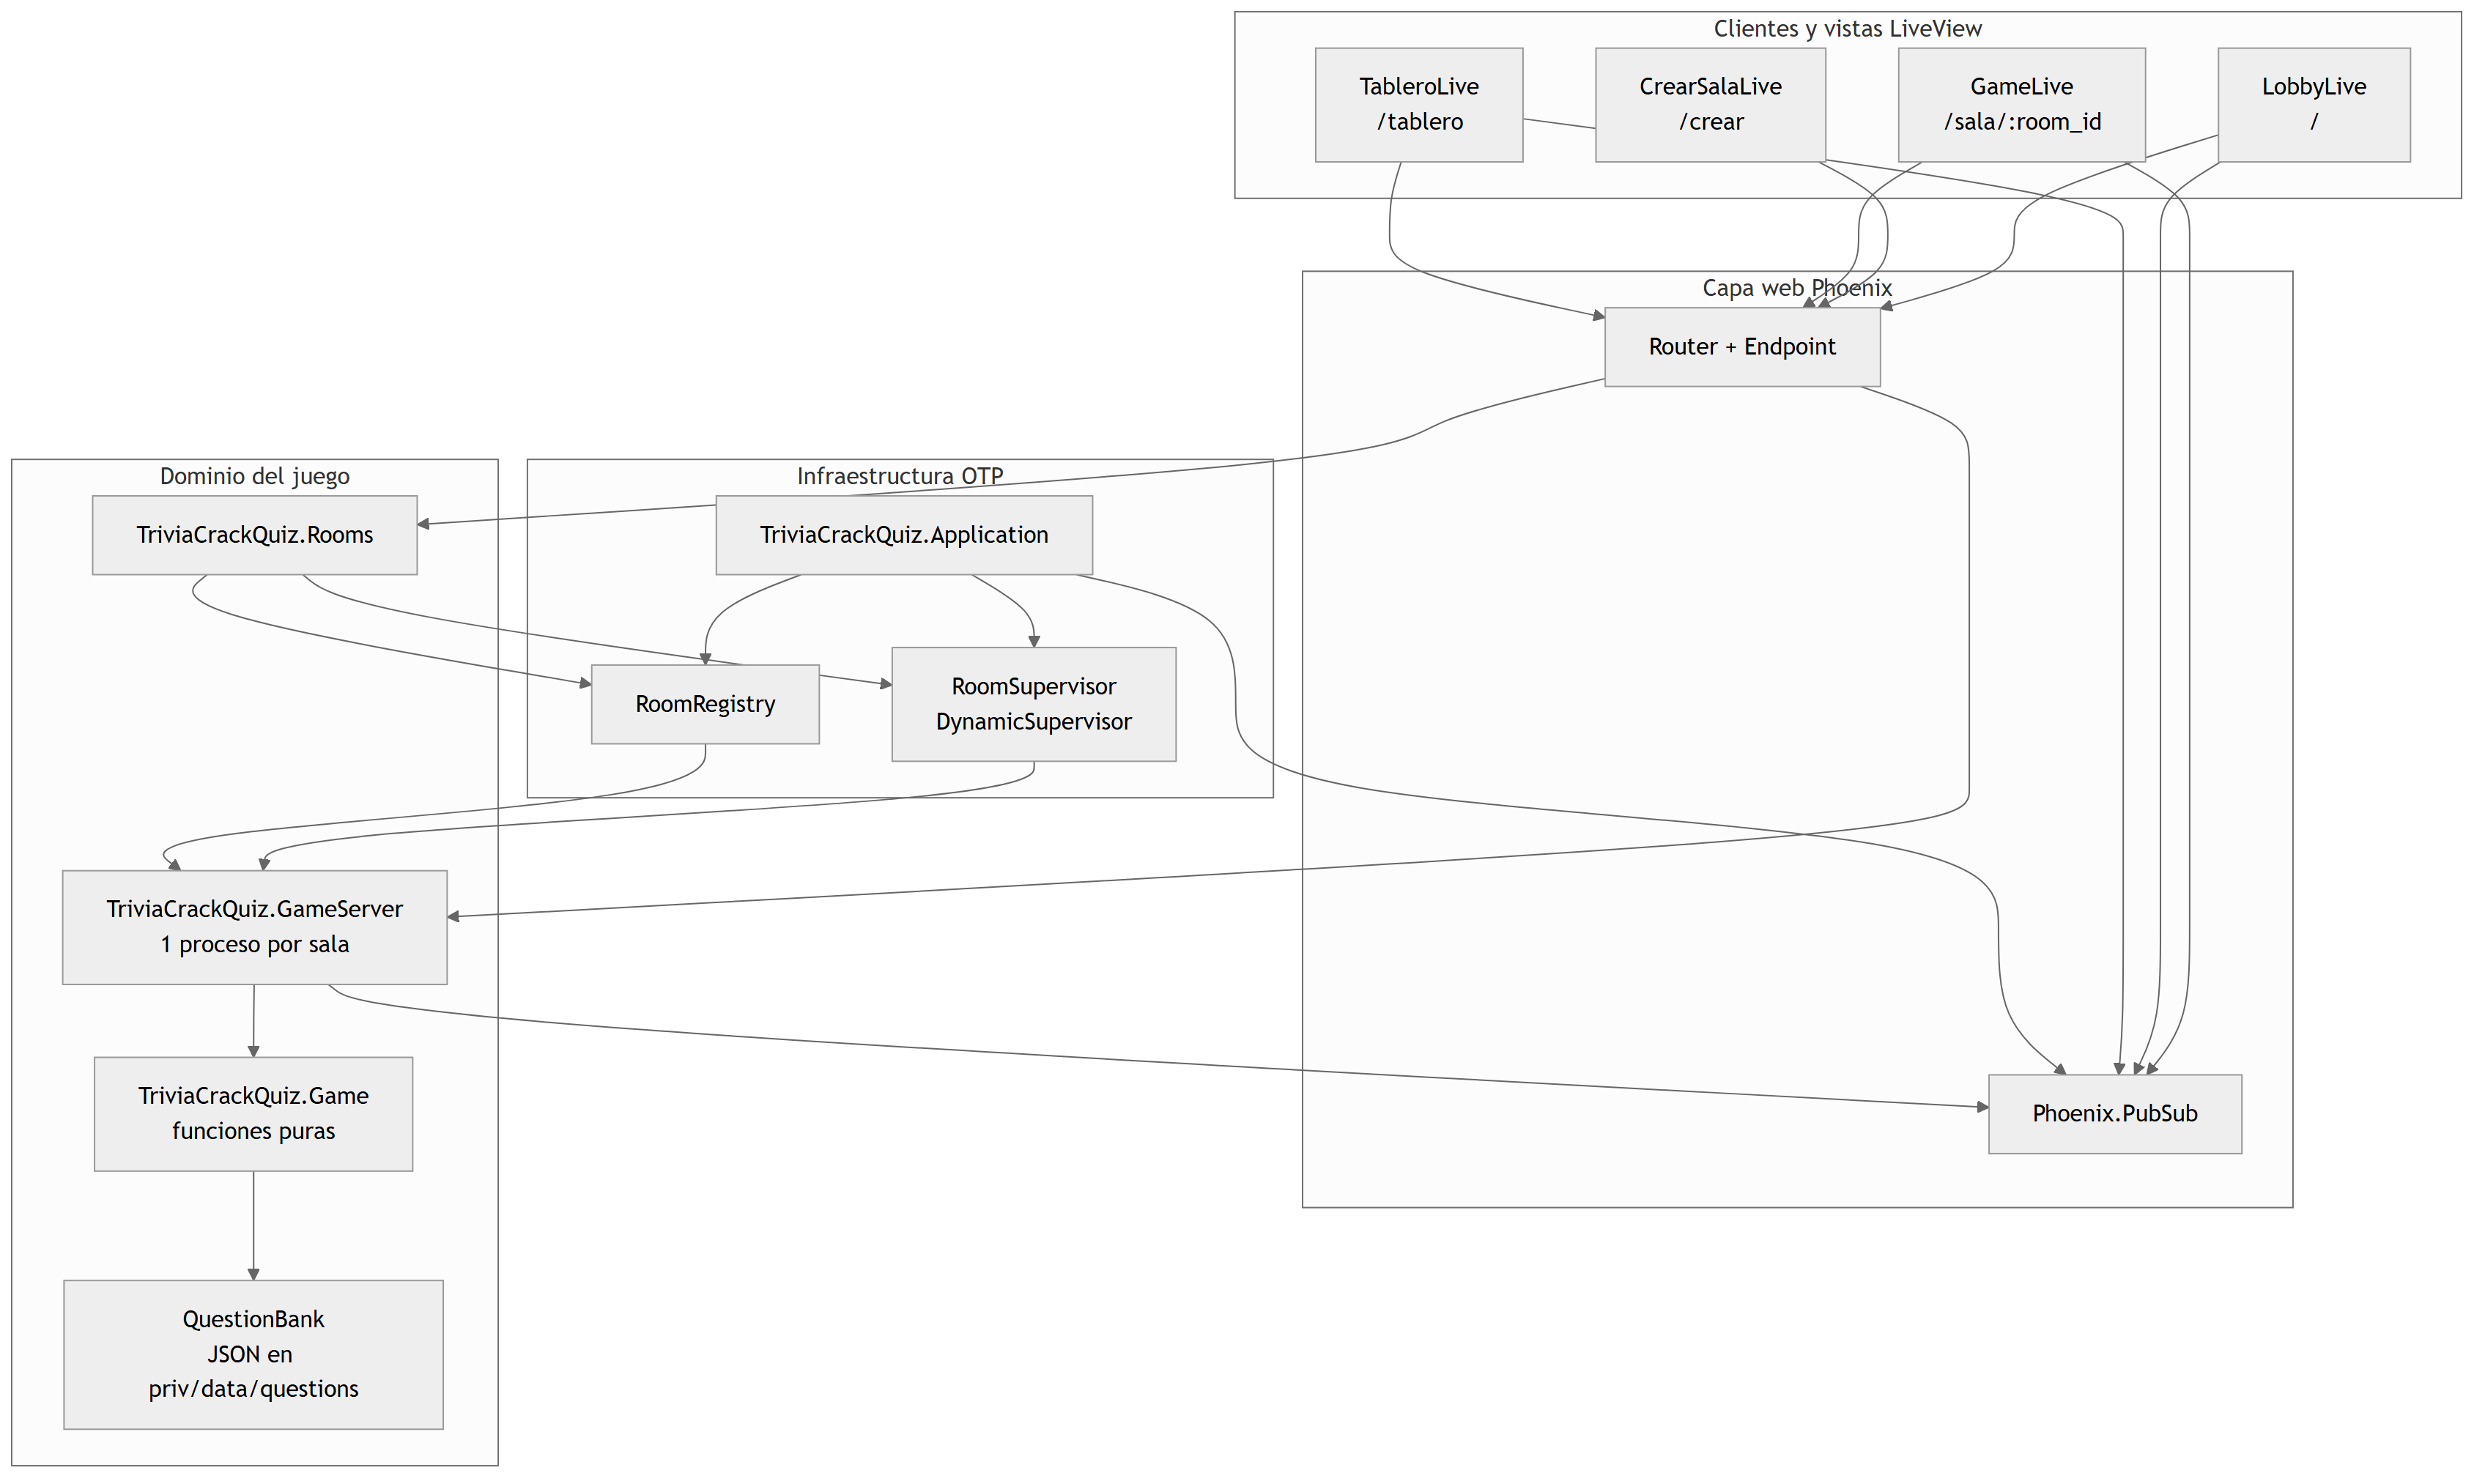
\includegraphics[width=\textwidth]{estructura_juego.png}
  \caption{Estructura general del juego y dependencias entre sus componentes.}
  \label{fig:estructura-juego}
\end{figure}

\subsection{Capas principales}

\begin{itemize}
  \item \textbf{Capa de interfaz:} los modulos \texttt{LobbyLive},
  \texttt{CrearSalaLive}, \texttt{GameLive} y \texttt{TableroLive} renderizan
  la interfaz y capturan eventos del navegador.
  \item \textbf{Capa de coordinacion:} \texttt{Rooms} crea, lista y cierra
  salas utilizando \texttt{DynamicSupervisor} y \texttt{Registry}.
  \item \textbf{Capa de procesos por sala:} \texttt{GameServer}
  mantiene el estado consistente de una partida, programa temporizadores y
  comunica cambios a los clientes.
  \item \textbf{Capa funcional pura:} \texttt{Game} concentra
  las reglas del juego como transformaciones de estado inmutables.
  \item \textbf{Datos de preguntas:} \texttt{QuestionBank}
  carga y normaliza el banco de preguntas desde \texttt{priv/data/questions/}.
\end{itemize}

\subsection{Arbol de supervision}

El modulo \texttt{TriviaCrackQuiz.Application} inicia los procesos globales que
permiten que la aplicacion funcione:

\begin{itemize}
  \item \texttt{TriviaCrackQuizWeb.Telemetry}
  \item \texttt{DNSCluster}
  \item \texttt{Phoenix.PubSub}
  \item \texttt{TriviaCrackQuiz.RoomRegistry}
  \item \texttt{TriviaCrackQuiz.RoomSupervisor}
  \item \texttt{TriviaCrackQuizWeb.Endpoint}
\end{itemize}

La estrategia \texttt{:one\_for\_one} garantiza que, si un proceso falla, solo
se reinicia ese proceso y no toda la aplicacion. Esta decision es esencial
porque evita que una falla en una sala interrumpa a las demas partidas activas.

\section{Estrategia de concurrencia y coordinacion en tiempo real}

La estrategia de concurrencia del proyecto se apoya por completo en Erlang/OTP
y en el paso de mensajes. En lugar de compartir un estado global mutable, cada
sala se representa como un proceso \texttt{GenServer} independiente identificado
por su \texttt{room\_id}. La Figura~\ref{fig:concurrencia-sala} describe el
flujo de eventos y actualizaciones dentro de una sala.

\begin{figure}[H]
  \centering
  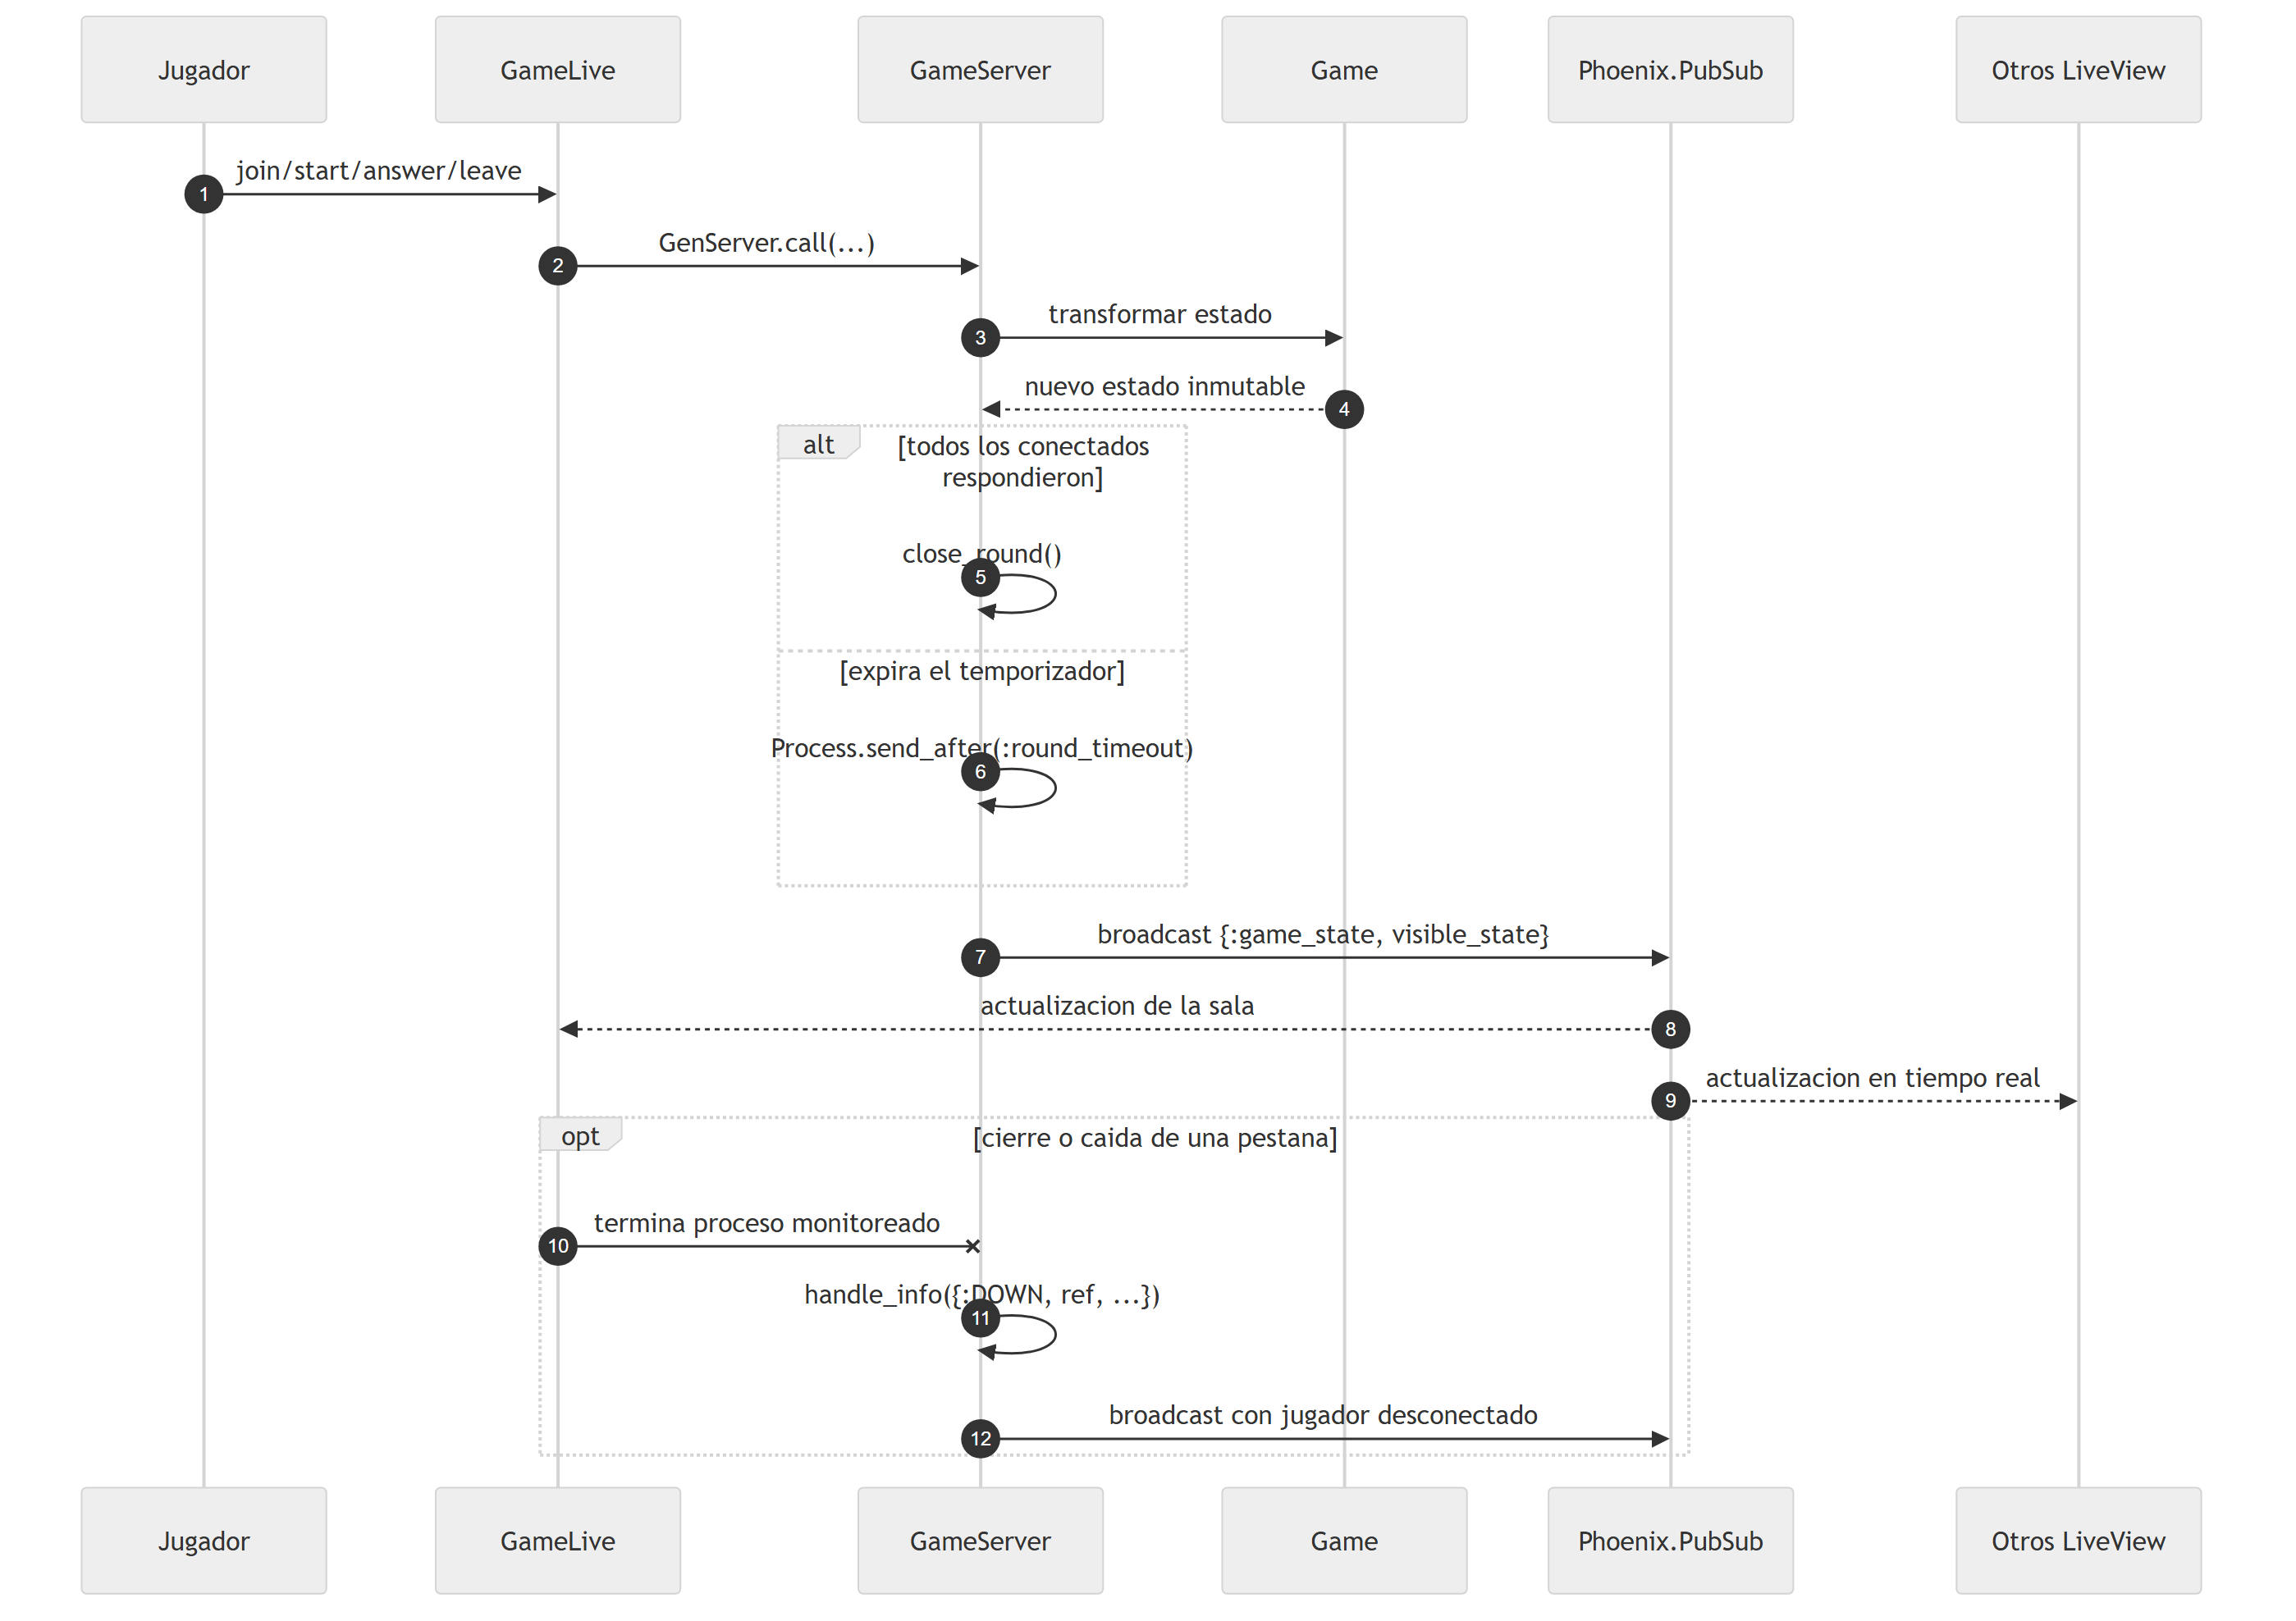
\includegraphics[width=\textwidth]{concurrencia_sala.png}
  \caption{Secuencia de concurrencia para una sala de juego.}
  \label{fig:concurrencia-sala}
\end{figure}

\subsection{Una sala equivale a un proceso}

Cuando un usuario crea una sala, \texttt{Rooms.create/2} solicita al
\texttt{RoomSupervisor} que inicie un hijo \texttt{GameServer}. Ese hijo queda
registrado en \texttt{RoomRegistry} mediante una clave unica basada en el
\texttt{room\_id}. A partir de ese momento:

\begin{itemize}
  \item todas las operaciones de la sala se encaminan al mismo proceso;
  \item el estado de la partida solo existe dentro de ese \texttt{GenServer};
  \item otras salas no pueden corromper ese estado porque no comparten memoria.
\end{itemize}

\subsection{Mensajes sincronizados y consistencia}

La capa web no modifica el estado del juego directamente. Los eventos del
usuario se traducen a llamadas como \texttt{join}, \texttt{start},
\texttt{answer}, \texttt{leave} o \texttt{reset}, que llegan al
\texttt{GameServer} mediante \texttt{GenServer.call/2}. Como un
\texttt{GenServer} atiende un mensaje a la vez, el estado se actualiza
secuencialmente y se evita la necesidad de bloqueos explicitos.

\subsection{PubSub para propagacion en tiempo real}

Despues de cada cambio, \texttt{GameServer} publica el estado visible mediante
\texttt{PubSub.broadcast/3}. Los LiveView suscritos al topico de esa sala
reciben el evento \texttt{:game\_state} y re-renderizan la interfaz. El lobby
general utiliza otro topico, \texttt{rooms}, para enterarse de altas, bajas o
cambios de estado de las salas.

\subsection{Temporizadores y eventos internos}

El flujo de la partida no depende solo de mensajes del usuario. El proceso de
la sala programa eventos internos con \texttt{Process.send\_after/3} para tres
casos:

\begin{itemize}
  \item \textbf{fin de ronda:} dispara \texttt{:round\_timeout} cuando se agota
  el tiempo de respuesta;
  \item \textbf{pantalla de resultados:} dispara \texttt{:results\_timeout}
  para avanzar automaticamente a la siguiente pregunta;
  \item \textbf{sala vacia:} dispara \texttt{:empty\_room\_timeout} cuando no
  queda ningun jugador conectado.
\end{itemize}

Esta estrategia evita depender de cron externos y concentra toda la logica
temporal dentro del actor que ya administra el estado de la sala.

\subsection{Monitoreo de jugadores y tolerancia a fallos}

Cada vez que un jugador entra o se reconecta, el \texttt{GameServer} monitorea
el proceso LiveView asociado. Si la pestana se cierra o el proceso termina, el
servidor recibe un mensaje \texttt{\{:DOWN, ref, :process, pid, reason\}} y
marca al jugador como desconectado. Este comportamiento permite:

\begin{itemize}
  \item conservar el puntaje del jugador aunque refresque la pagina;
  \item no bloquear la partida esperando respuestas de clientes desconectados;
  \item cerrar automaticamente una sala abandonada sin afectar al resto del
  sistema.
\end{itemize}

\section{Definicion de modulos y funciones principales}

Las funciones importantes del sistema se organizan por responsabilidad, no por
orden de archivo. Los modulos mas relevantes son los siguientes:

\begin{description}
  \item[\texttt{TriviaCrackQuiz.Application}] Arranque OTP. Define el arbol de
  supervision, inicia PubSub, Registry, DynamicSupervisor y el Endpoint web.
  \item[\texttt{TriviaCrackQuiz.Rooms}] Gestor de salas. Crea, lista, cierra y
  busca salas; tambien notifica al lobby cuando cambia el conjunto de partidas
  activas.
  \item[\texttt{TriviaCrackQuiz.GameServer}] Actor por sala. Mantiene el estado
  de una partida, procesa mensajes, controla timers y difunde actualizaciones
  en tiempo real.
  \item[\texttt{TriviaCrackQuiz.Game}] Motor funcional puro. Implementa reglas
  del juego: altas de jugadores, rondas, filtros, puntaje, respuestas
  correctas y cierre de partida.
  \item[\texttt{TriviaCrackQuiz.QuestionBank}] Proveedor de datos. Carga y
  normaliza preguntas desde archivos JSON del proyecto.
  \item[\texttt{TriviaCrackQuizWeb.GameLive}] Vista interactiva. Presenta el
  estado de la sala y traduce acciones del navegador en eventos de servidor.
\end{description}

\subsection{Creacion y administracion de salas}

\texttt{Rooms} concentra la administracion del ciclo de vida de las salas:

\begin{itemize}
  \item \texttt{create/2}: arranca una sala con filtros opcionales y devuelve
  un \texttt{room\_id} estable.
  \item \texttt{create\_random/1}: genera un identificador legible y crea una
  sala nueva.
  \item \texttt{create\_named/2}: transforma un nombre escrito por el usuario
  en un identificador apto para URL.
  \item \texttt{random\_open/1}: localiza una sala en espera con filtros
  compatibles o crea una nueva si no existe.
  \item \texttt{list/0}: construye un resumen de las salas activas para el
  lobby y el tablero espectador.
  \item \texttt{close/1}: termina el proceso de una sala cuando deja de ser
  necesaria.
\end{itemize}

Estas funciones encapsulan el uso de \texttt{DynamicSupervisor} y
\texttt{Registry}, de modo que el resto del sistema nunca trabaja con pids de
forma manual.

\subsection{Ciclo de vida de la partida}

El modulo \texttt{Game} define la logica del juego como transformaciones puras
de un mapa de estado:

\begin{itemize}
  \item \texttt{new\_state/2}: crea el estado inicial con filtros, tiempos,
  ronda sorpresa y banco de preguntas disponible.
  \item \texttt{add\_player/3} y \texttt{remove\_player/2}: agregan o eliminan
  jugadores sin romper la inmutabilidad del estado.
  \item \texttt{start/1}: valida que exista el minimo de jugadores e inicia la
  primera ronda.
  \item \texttt{next\_question/1}: selecciona una pregunta, actualiza la ronda
  actual y reinicia respuestas pendientes.
  \item \texttt{register\_answer/3}: registra la respuesta de un jugador junto
  con el instante exacto en que respondio.
  \item \texttt{evaluate\_round/1}: decide si cada respuesta es correcta,
  calcula puntaje y genera la estructura de resultados de la ronda.
  \item \texttt{reset/1}, \texttt{reopen\_room/1} y \texttt{finish/1}: reinician
  o cierran la partida segun el estado alcanzado.
\end{itemize}

La funcion \texttt{visible\_state/1} cumple un papel de seguridad importante:
antes de enviar el estado al navegador elimina respuestas correctas, timers,
monitores y datos internos que no deben exponerse al cliente.

\subsection{Seleccion de preguntas, filtros y validacion de respuestas}

El juego no usa una base de datos; las preguntas se cargan desde archivos JSON
en \texttt{priv/data/questions/}. Las funciones clave para esta parte son:

\begin{itemize}
  \item \texttt{QuestionBank.load\_questions/0}: lee y normaliza el banco de
  preguntas del proyecto.
  \item \texttt{Game.available\_categories/1} y \texttt{available\_types/1}:
  extraen las opciones disponibles para los formularios de creacion de sala.
  \item \texttt{Game.correct\_answer?/2}: compara la respuesta enviada por el
  usuario contra la respuesta oficial y alternativas aceptadas.
  \item \texttt{Game.question\_time\_ms/1}: ajusta la duracion de la ronda segun
  el tipo de pregunta.
\end{itemize}

En preguntas de tipo \texttt{:quick\_answer}, la validacion tolera errores de
tipeo pequenos mediante una implementacion propia de distancia de Levenshtein.
Esta decision mejora la experiencia de juego sin desordenar la capa de
presentacion.

\subsection{Publicacion de estado a los clientes}

\texttt{GameServer} conecta la logica funcional con la
infraestructura concurrente:

\begin{itemize}
  \item \texttt{join/3}, \texttt{reconnect/2}, \texttt{leave/2},
  \texttt{start\_game/1}, \texttt{answer/3} y \texttt{reset/1} representan la
  API publica de una sala.
  \item \texttt{handle\_call/3} serializa las operaciones solicitadas por los
  clientes y delega cada decision de negocio al modulo \texttt{Game}.
  \item \texttt{handle\_info/2} procesa expiracion de timers y eventos
  \texttt{:DOWN} provenientes del monitoreo de jugadores.
  \item \texttt{broadcast\_state/1} publica la vista saneada del estado mediante
  PubSub para actualizar clientes y tablero.
\end{itemize}

\section{Decisiones funcionales y de diseno}

El proyecto fue construido bajo lineamientos del paradigma funcional, y eso se
refleja en varias decisiones de implementacion:

\begin{itemize}
  \item \textbf{Inmutabilidad:} las reglas del juego no mutan estructuras en el
  lugar; siempre devuelven un nuevo mapa de estado.
  \item \textbf{Funciones puras:} \texttt{TriviaCrackQuiz.Game} no conoce
  sockets, procesos ni PubSub. Solo transforma datos.
  \item \textbf{Separacion de efectos:} \texttt{GameServer} concentra IO,
  temporizadores, monitoreo y mensajeria, mientras el motor funcional decide
  reglas.
  \item \textbf{Pattern matching y guards:} el flujo del programa distingue
  estados validos directamente en las cabeceras de funciones, por ejemplo al
  evaluar rondas o procesar timeouts.
  \item \textbf{Paso de mensajes en lugar de locks:} la coherencia se garantiza
  al procesar un mensaje por vez dentro del actor de la sala.
\end{itemize}

Esta separacion mejora la mantenibilidad: las pruebas del dominio pueden
ejecutarse sin levantar la interfaz web, mientras que la capa concurrente puede
probarse como comportamiento de actores reales.

\section{Flujo operativo de una partida}

El comportamiento del sistema puede resumirse en la siguiente secuencia:

\begin{enumerate}
  \item Un jugador entra al lobby y crea una sala o solicita union aleatoria.
  \item \texttt{Rooms} crea o localiza el \texttt{GameServer} correspondiente.
  \item \texttt{GameLive} se suscribe al topico \texttt{game:room:<room\_id>}.
  \item Los jugadores se registran, el servidor monitorea sus procesos y el
  lobby recibe notificaciones de cambio de aforo.
  \item Cuando hay al menos tres jugadores, uno de ellos inicia la partida.
  \item Cada respuesta entra al \texttt{GameServer}, que actualiza el estado
  mediante funciones puras y recalcula si la ronda debe cerrarse.
  \item El proceso difunde el nuevo estado y todos los clientes de la sala ven
  el mismo resultado en tiempo real.
  \item Tras la ronda final, la partida muestra podio y ganador, y puede
  reiniciarse o cerrarse.
\end{enumerate}

\section{Conclusion}

La arquitectura del proyecto demuestra que es posible construir un juego
multijugador coherente y extensible usando principios funcionales y
concurrencia basada en actores. El uso de Phoenix LiveView reduce la complejidad
de sincronizacion en el cliente, mientras que OTP ofrece aislamiento de fallos,
supervision y procesos ligeros para modelar cada sala como una unidad
independiente.

El resultado es un sistema adecuado para entregas academicas y para evolucionar
tecnicamente: admite nuevas categorias de preguntas, ajustes de puntaje,
persistencia futura o nuevas vistas sin romper la separacion entre dominio,
procesos y presentacion.

\vspace{1cm}
\noindent\textbf{Nota de mantenimiento.} Este documento se complementa con la
guia ubicada en \path{docs/guia_instalacion_local.md}, donde se detallan los
pasos para clonar el repositorio, ejecutar el proyecto y regenerar el PDF de
esta documentacion tecnica.

\end{document}
